\documentclass{article}
\usepackage[utf8]{inputenc}
\usepackage[T1]{fontenc}

\usepackage{amsmath,amsthm,graphicx,amssymb,float,authblk,color,subcaption,appendix,bm}
\captionsetup[subfigure]{labelformat=simple}
\usepackage{algorithm,algpseudocode}
\usepackage{url,hyperref}
\usepackage[round]{natbib}
\usepackage[sc]{mathpazo}
\usepackage[gen]{eurosym}
% \usepackage{biblatex}
\usepackage[capitalise]{cleveref}
\usepackage[dvipsnames]{xcolor}
\usepackage{placeins}

%%%%%%%%%% EXACT 1in MARGINS %%%%%%%                                   %%
\setlength{\textwidth}{6.5in}     %%                                   %%
\setlength{\oddsidemargin}{0in}   %% (It is recommended that you       %%
\setlength{\evensidemargin}{0in}  %%  not change these parameters,     %%
\setlength{\textheight}{9in}      %%  at the risk of having your       %%0
%\setlength{\topmargin}{0.5in}       %%  proposal dismissed on the basis  %%
\setlength{\headheight}{-0.4in}      %%  of incorrect formatting!!!)      %%
\setlength{\headsep}{0.1in}         %%

% Notations
\newcommand{\setK}{\mathcal{K}}
\newcommand{\setA}{\mathcal{A}}
\newcommand{\setB}{\mathcal{B}}
\newcommand{\setI}{\mathcal{I}}
\newcommand{\mbbone}{\mathbb{1}}

% environments
\newtheorem{proposition}{Proposition}
\newtheorem{theorem}{Theorem}
\newtheorem{lemma}{Lemma}
\newtheorem{definition}{Definition}
\newtheorem{corollary}{Corollary}
\newtheorem{assumption}{Assumption}
\newtheorem{remark}{Remark}

% Comments
\newcommand{\kz}[1]{{\color{magenta}{\noindent #1}}}
\newcommand{\jl}[1]{{\color{blue}{\noindent #1}}}



\title{Optimistic and Pessimistic Mobility-as-a-Service Bundle Design}

\begin{document}

\maketitle

\section{Introduction}

\jl{What is real bunlde and why it's hard}

The inherent difficulty of bundle design has led existing studies to rely on substantial simplifications.

In the MaaS model of \citet{LiEtAlMaaSContinuous}, trip frequency directly indexes traveler heterogeneity and provides a natural axis for bundle segmentation, leading to a structure similar to continuous-type heterogeneous user equilibrium models \citep{dial1996,xie2026,Wang2026,xu2026}. This structure gives the lower-level problem favorable properties and allows travelers to be ordered exactly by trip frequency. However, using trip frequency itself as the source of traveler heterogeneity is behaviorally restrictive. In practice, an individual traveler's trip frequency is uncertain over the bundle horizon, rather than being a fixed characteristic that uniquely defines the traveler's type. It is therefore more natural to model travelers as heterogeneous classes, while allowing trip frequency to vary randomly within each class.

\subsection{Main ideas}
\begin{itemize}
    \item Finite number of user classes, while each class features a continuous trip frequency distribution, e.g., daily commuters vs flexible working schedules
    \item Travelers in each class make bundle choice based on some statistical metric of generalized path cost (e.g., expectation).
    \item Expected travel flows are constrained by bundle-specific link capacity constraints, while the shadow price of each constraint is included in the generalized path cost.
    \item Design variables of each bundle are the bundle price and maximum usage of each mode, i.e., the set of link capacities.
    \item Expected outcomes: travelers with different trip frequency distributions and feasible paths vary in their bundle preferences. Hence, bundle design introduces a form of service personalization instead of simply price discrimination.
\end{itemize}

\section{MaaS Bundle Design under Uncertainty}

\subsection{Bundle Setting}

A MaaS bundle combines a subscription fee with prepaid allowances and overage charges. Because travelers can satisfy their mobility demand through different transport modes, both the included quantities and the excess-usage charges are specified by mode. We therefore model each bundle as a multidimensional three-part tariff.

Let $i\in\mathcal I$, $b\in\mathcal B$, and $m\in\mathcal M$ index traveler classes, subscription bundles, and transport modes, respectively. Each subscription bundle $b\in\mathcal B$ is characterized by a subscription fee $C_b\geq 0$, a vector of mode-specific allowances $\varepsilon_b\in\mathbb{R}_+^{|\mathcal M|}$, and a vector of strictly positive per-unit overage charges $\rho\in\mathbb{R}_{++}^{|\mathcal M|}$. The overage component can be interpreted as pay-as-you-go (PAYG) access for usage beyond the included allowances. As a limiting case, pure PAYG, corresponding to non-subscribers, is represented as a zero-fee bundle with zero included allowances. We index this option by $b=0$ and define $\mathcal B_0:=\{0\}\cup\mathcal B$ as the complete bundle menu, with $C_0=0$ and $\varepsilon_0=0$.

Travelers therefore trade off prepaid allowances against future possible PAYG usage. This trade-off varies across traveler classes because they differ in both their feasible path sets and trip-frequency distributions. Trip frequency,  denoted as $\mu$, is typically unknown when a bundle is selected. We therefore model it as a random variable whose distribution $F_i$ is known to the traveler class $i$. Ultimately, travelers compare bundles by combining the subscription fee with the expected minimum travel cost (EMTC) under these distributions.

\subsection{Ex Post Travel Allocation}

We begin with travelers' path allocation after the trip frequency is realized.

Consider a class-$i$ traveler who has selected bundle $b\in\setB$ and travels over a network with link set $\mathcal A$ using the transport modes in $\mathcal M$. After the trip frequency $\mu\sim F_i$ is realized, the traveler allocates the resulting trips across the feasible path set $P_{ib}$. Let $f_{ib}(\mu)\in\mathbb{R}_+^{|P_{ib}|}$ denote the path usage vector, satisfying
\begin{equation}
    \mbbone^\top f_{ib}(\mu)=\mu.
    \label{eq:path-usage-conservation}
\end{equation}
The corresponding link usage vector is
$x_{ib}(\mu)=\Delta_{ib}f_{ib}(\mu)$, where $\Delta_{ib}$ is the link--path incidence matrix. Similarly, given the link travel time vector $t\in\mathbb{R}_+^{|\mathcal A|}$, the corresponding path travel time vector is
$\bar c_{ib}:=\Delta_{ib}^\top t$.

Unlike physical link capacities, the allowances included in a MaaS bundle do not restrict whether a path can be used. Instead, they determine which portion of the resulting mode usage is covered by the subscription and which portion incurs overage charges. Because a path may involve multiple transport modes, its use may draw simultaneously on several mode-specific allowances. The bundle's allowance structure must therefore be incorporated explicitly into the path allocation model.

To represent mode usage, let
\[
N_{ib}\in\mathbb{R}_+^{|\mathcal M|\times |P_{ib}|}
\]
denote the mode--path usage matrix, whose $(m,p)$th element gives the amount of mode $m$ used by one trip on path $p\in P_{ib}$. The aggregate mode usage induced by the path allocation $f_{ib}(\mu)$ is therefore $N_{ib}f_{ib}(\mu)$. We introduce the excess-usage vector
$z_{ib}(\mu)\in\mathbb{R}_+^{|\mathcal M|}$ through
\begin{equation}
    N_{ib}f_{ib}(\mu)
    \leq
    \varepsilon_b+z_{ib}(\mu).
    \label{eq:mode-allowance}
\end{equation}
When excess usage is subject to strictly positive overage charges, $z_{ib}(\mu)$ takes its smallest feasible value and thus represents the mode usage beyond the included allowances.

Conditional on the realized trip frequency $\mu$, the traveler selects the path allocation and excess usage by solving
\begin{equation}
\label{eq:realized-path-allocation}
\begin{aligned}
\Phi_{ib}(\mu;\bm\varepsilon_b,\bm\rho)
:=
\min_{\bm f_{ib},\,\bm z_{ib}}
\quad&
\beta\,\bar{\bm c}_{ib}^{\top}\bm f_{ib}
+
\bm\rho^{\top}\bm z_{ib}
\\
\text{s.t.}\quad&
\eqref{eq:path-usage-conservation},
\quad
\eqref{eq:mode-allowance},
\\
&
\bm f_{ib}\geq\bm 0,
\qquad
\bm z_{ib}\geq\bm 0.
\end{aligned}
\end{equation}
The first term in the objective represents the monetary value of the total travel time incurred over the bundle period, while the second term represents the total PAYG expenditure for mode usage exceeding the included allowances. Let
$
\bigl(f_{ib}^*(\mu),z_{ib}^*(\mu)\bigr)
$
denote an optimal solution to problem~\eqref{eq:realized-path-allocation}. Its optimal value
$\Phi_{ib}(\mu;\varepsilon_b,\rho)$ is the minimum ex post travel cost incurred by a class-$i$ traveler under option $b$ and realization $\mu$.

\begin{remark}[Interpretation of the allowance constraint] Constraint~\eqref{eq:mode-allowance} can equivalently be interpreted as imposing a hard upper bound on the mode usage covered by the bundle, with any remaining usage purchased through PAYG. Specifically, by introducing $u_{ib}(\mu)\in\mathbb{R}_+^{|\mathcal M|}$, it can be written as $N_{ib}f_{ib}(\mu)=u_{ib}(\mu)+z_{ib}(\mu)$ and $0\leq u_{ib}(\mu)\leq\varepsilon_b$, where $u_{ib}(\mu)$ and $z_{ib}(\mu)$ represent bundle-covered and PAYG mode usage, respectively. \end{remark}

\subsection{Ex Ante Bundle Choice}

Travelers select a bundle before their trip frequency is realized. They therefore evaluate each option according to the EMTC induced by their class-specific trip-frequency distribution. For traveler class $i\in\mathcal I$ and option $b\in\mathcal B_0$, define the generalized bundle cost as
\begin{equation}
e_{ib}
=
C_b
+
\mathbb E_{\mu\sim F_i}
\left[
\Phi_{ib}(\mu;\varepsilon_b,\rho)
\right],
\label{eq:bundle-generalized-cost}
\end{equation}
where $C_b$ is the subscription fee.

Let $\Pi_i:=\min_{b\in\mathcal B_0} e_{ib}$
denote the minimum generalized cost attainable by class $i$, and define the corresponding set of minimum-cost options as
\begin{equation}
\mathcal B_i^*
:=
\arg\min_{b\in\mathcal B_0} e_{ib}.
\label{eq:min-cost-bundle-set}
\end{equation}

Let $q_{ib}$ denote the fraction of class-$i$ travelers choosing option $b$. The bundle-choice conditions are
\begin{align}
&q_{ib}\geq 0,
\qquad
\sum_{b\in\mathcal B_0}q_{ib}=1,
\label{eq:bundle-choice-simplex}\\
&0\leq q_{ib}
\perp
e_{ib}-\Pi_i
\geq0,
\qquad
b\in\mathcal B_0.
\label{eq:bundle-choice-complementarity}
\end{align}
The complementarity condition implies that an option can receive a positive share of class-$i$ travelers only if it attains the minimum generalized cost. Equivalently,
\begin{equation}
q_{ib}>0
\quad\Longrightarrow\quad
b\in\mathcal B_i^*.
\end{equation}

In the flow-independent setting considered here, the generalized bundle costs are independent of the bundle shares. Hence, if $\mathcal B_i^*$ is a singleton, the entire traveler class selects the unique minimum-cost option, and the resulting choice vector $q_i$ is a vertex of the probability simplex. In this case, the class-level bundle choice is effectively binary. If several options attain the same minimum generalized cost, however, the choice correspondence is set-valued: any choice vector supported on $\mathcal B_i^*$ satisfies \eqref{eq:bundle-choice-simplex}--\eqref{eq:bundle-choice-complementarity}.

\subsection{Bundle Design Problem}

We now formulate the platform's bundle design problem. Taking the
mode-specific overage tariffs $\bm\rho$ as given, the platform jointly
chooses the subscription fees $\bm C:=(C_b)_{b\in\mathcal B}$ and
allowance vectors $\bm\varepsilon:=(\bm\varepsilon_b)_{b\in\mathcal B}$.

Let $Q_i$ denote the size of traveler class $i$. For each subscription
bundle $b\in\mathcal B$, let $K_b(\bm\varepsilon_b)$ denote the nonnegative,
continuous provision cost per subscriber, with $K_b(\bm0)=0$. We assume
that $K_b$ is continuously differentiable wherever derivative information
is used. The platform margin from a traveler selecting option $b\in\mathcal B_0$ is
\begin{equation}
    M_b(C_b,\bm\varepsilon_b)
    :=
    C_b-K_b(\bm\varepsilon_b).
    \label{eq:bundle-margin}
\end{equation}

For a given menu $(\bm C,\bm\varepsilon)$, define the optimal-response set
of traveler class $i$ as
\begin{equation}
    \mathcal S_i(\bm C,\bm\varepsilon)
    :=
    \arg\min_{\bm q_i\geq\bm0}
    \left\{
        \sum_{b\in\mathcal B_0}
        q_{ib}e_{ib}(\bm C,\bm\varepsilon):
        \sum_{b\in\mathcal B_0}q_{ib}=1
    \right\}.
    \label{eq:bundle-choice-solution-set}
\end{equation}

Among these minimum-cost responses, the optimistic and pessimistic rules
select those that maximize and minimize the platform margin, respectively:
\begin{align}
    \mathcal S_i^{\mathrm O}(\bm C,\bm\varepsilon)
    &:=
    \arg\max_{\bm q_i\in\mathcal S_i(\bm C,\bm\varepsilon)}
    \sum_{b\in\mathcal B_0}
    q_{ib}M_b(C_b,\bm\varepsilon_b),
    \label{eq:optimistic-response-set}\\
    \mathcal S_i^{\mathrm P}(\bm C,\bm\varepsilon)
    &:=
    \arg\min_{\bm q_i\in\mathcal S_i(\bm C,\bm\varepsilon)}
    \sum_{b\in\mathcal B_0}
    q_{ib}M_b(C_b,\bm\varepsilon_b).
    \label{eq:pessimistic-response-set}
\end{align}

Let $\mathcal D$ denote the feasible set of bundle menus:
\begin{equation}
\begin{aligned}
    \mathcal D
    :=
    \bigl\{
    (\bm C,\bm\varepsilon):
    \;& C_b\geq0,\quad
       \bm\varepsilon_b\geq\bm0,
       && b\in\mathcal B,\\
    & C_{b+1}\geq C_b,
       && b=1,\ldots,B-1,\\
    & C_0=0,\quad
      \bm\varepsilon_0=\bm0
    \bigr\}.
\end{aligned}
\label{eq:bundle-menu-feasible-set}
\end{equation}

For a given selection rule $r\in\{\mathrm O,\mathrm P\}$, the platform's
bundle design problem is
\begin{align}
    \max_{\bm C,\bm\varepsilon,\bm q}
    \quad&
    \sum_{i\in\mathcal I}
    Q_i
    \sum_{b\in\mathcal B_0}
    q_{ib}M_b(C_b,\bm\varepsilon_b)
    \label{eq:bundle-design-objective}\\
    \text{s.t.}\quad&
    \bm q_i\in
    \mathcal S_i^r(\bm C,\bm\varepsilon),
    && i\in\mathcal I,
    \label{eq:bundle-design-response}\\
    &
    (\bm C,\bm\varepsilon)\in\mathcal D.
    \label{eq:bundle-design-menu}
\end{align}
We refer to the cases $r=\mathrm O$ and $r=\mathrm P$ as optimistic bundle
design (OBD) and pessimistic bundle design (PBD), respectively. The two selection rules can differ only when a traveler class has multiple minimum-cost options.


\section{Bundle Valuation and Segmentation}
\label{sec:bundle-valuation-segmentation}

\subsection{Bundle Valuation and Marginal Allowance Value}
\label{sec:bundle-valuation}

We first express the EMTC separately from the subscription fee. For
traveler class $i$ and bundle $b$, define
\begin{equation}
    G_{ib}(\bm\varepsilon_b)
    :=
    \mathbb E_{\mu\sim F_i}
    \left[
        \Phi_{ib}(\mu;\bm\varepsilon_b,\bm\rho)
    \right].
    \label{eq:expected-route-cost}
\end{equation}

For any realization $\mu$, strong duality gives
\begin{align}
    \Phi_{ib}(\mu;\bm\varepsilon_b,\bm\rho)
    =
    \max_{\pi_{ib},\bm\omega_{ib}}
    \quad&
    \mu\pi_{ib}
    -
    \bm\omega_{ib}^{\top}\bm\varepsilon_b
    \label{eq:route-dual-objective}\\
    \text{s.t.}\quad&
    \pi_{ib}\bm 1
    -
    N_{ib}^{\top}\bm\omega_{ib}
    \leq
    \beta\bar{\bm c}_{ib},
    \label{eq:route-dual-path}\\
    &
    \bm0\leq\bm\omega_{ib}\leq\bm\rho.
    \label{eq:route-dual-shadow}
\end{align}
The variable $\pi_{ib}$ represents the minimum generalized path cost
under the allowance shadow prices and is free in the dual. An optimal
solution can, however, always be chosen with $\pi_{ib}\geq0$. The point
$(\pi_{ib},\bm\omega_{ib})=(0,\bm0)$ is feasible and gives zero
objective value. Any feasible solution with $\pi_{ib}<0$ gives a
nonpositive objective value. We can therefore impose
$\pi_{ib}\geq0$ without changing the optimal value.

The shadow price $\omega_{ib,m}$ measures the marginal value of the
allowance for mode $m$. The dual constraint
$0\leq\omega_{ib,m}\leq\rho_m$ also gives a direct bound on this
value. One additional unit of allowance can save at most one unit of
the corresponding PAYG charge. Its marginal value therefore cannot
exceed $\rho_m$.

A key feature of the dual problem is that its constraints do not depend
on $\mu$ or $\bm\varepsilon_b$. These two terms appear only in the
objective. We therefore define the common dual feasible region as
\begin{equation}
    \mathcal V_{ib}
    :=
    \left\{
        (\pi,\bm\omega):
        \pi\bm 1-N_{ib}^{\top}\bm\omega
        \leq
        \beta\bar{\bm c}_{ib},
        \;
        \pi\geq0,
        \;
        \bm0\leq\bm\omega\leq\bm\rho
    \right\}.
    \label{eq:dual-feasible-region}
\end{equation}

\begin{lemma}
For each traveler class $i$ and bundle $b$, the set
$\mathcal V_{ib}$ is a polytope that is independent of the
trip-frequency realization $\mu$ and the allowance vector
$\bm\varepsilon_b$. Let $\mathcal J_{ib}$ index the extreme points
$(\pi_{ib}^j,\bm\omega_{ib}^j)$ of $\mathcal V_{ib}$. Then, for every
$\mu$ and $\bm\varepsilon_b$,
\begin{equation}
    \Phi_{ib}(\mu;\bm\varepsilon_b,\bm\rho)
    =
    \max_{j\in\mathcal J_{ib}}
    \left\{
        \pi_{ib}^j\mu
        -
        (\bm\omega_{ib}^j)^{\top}\bm\varepsilon_b
    \right\}.
    \label{eq:route-value-vertex}
\end{equation}
\label{lem:fixed-dual-geometry}
\end{lemma}

\begin{proof}
The constraints that define $\mathcal V_{ib}$ contain neither $\mu$
nor $\bm\varepsilon_b$. Hence, the feasible region is unchanged when
these parameters vary.

The vector $\bm\omega$ is bounded by $\bm\rho$. The path constraints
then give an upper bound on $\pi$. Thus, $\mathcal V_{ib}$ is bounded.
Since it is defined by finitely many linear inequalities,
$\mathcal V_{ib}$ is a polytope.

The dual objective is linear in $(\pi,\bm\omega)$. An optimal solution
is therefore attained at an extreme point of $\mathcal V_{ib}$. This
gives~\eqref{eq:route-value-vertex}.
\end{proof}

Lemma~\ref{lem:fixed-dual-geometry} also gives the shape of the minimum
ex post travel cost.

\begin{corollary}
For each traveler class $i$ and bundle $b$,
$\Phi_{ib}(\mu;\bm\varepsilon_b,\bm\rho)$ is jointly convex and
piecewise linear in $(\mu,\bm\varepsilon_b)$. It is nondecreasing in
$\mu$ and componentwise nonincreasing in $\bm\varepsilon_b$.
\label{cor:realized-valuation-properties}
\end{corollary}

\begin{proof}
By~\eqref{eq:route-value-vertex}, $\Phi_{ib}$ is the maximum of a finite
number of affine functions of $(\mu,\bm\varepsilon_b)$. It is therefore
convex and piecewise linear. Since $\pi_{ib}^j\geq0$ for every
$j\in\mathcal J_{ib}$, it is nondecreasing in $\mu$. Since
$\bm\omega_{ib}^j\geq\bm0$, it is componentwise nonincreasing in
$\bm\varepsilon_b$.
\end{proof}

Within a region where extreme point $j^*$ is uniquely optimal, the minimum
ex post travel cost is
\begin{equation}
    \Phi_{ib}(\mu;\bm\varepsilon_b,\bm\rho)
    =
    \pi_{ib}^{j^*}\mu
    -
    (\bm\omega_{ib}^{j^*})^{\top}\bm\varepsilon_b.
    \label{eq:route-value-local-affine}
\end{equation}
Thus, $-\bm\omega_{ib}^{j^*}$ gives the local marginal effect of the
allowance vector. This effect changes only when the optimal dual
extreme point changes.

We now consider the EMTC
$G_{ib}(\bm\varepsilon_b)$.

\begin{proposition}
Suppose that $F_i$ has a finite mean. Then
$G_{ib}(\bm\varepsilon_b)$ is finite, convex, and componentwise
nonincreasing. Moreover, for any
$\bm\varepsilon_b,\bm\varepsilon_b'\geq\bm0$,
\begin{equation}
    \left|
        G_{ib}(\bm\varepsilon_b')
        -
        G_{ib}(\bm\varepsilon_b)
    \right|
    \leq
    \bm\rho^{\top}
    \left|
        \bm\varepsilon_b'
        -
        \bm\varepsilon_b
    \right|.
    \label{eq:valuation-lipschitz}
\end{equation}
\label{prop:expected-valuation-properties}
\end{proposition}

\begin{proof}
For each realization $\mu$,
Corollary~\ref{cor:realized-valuation-properties} shows that
$\Phi_{ib}$ is convex and componentwise nonincreasing in
$\bm\varepsilon_b$. Taking expectations preserves both properties.
Since the dual feasible region is bounded, the optimal path cost grows
at most linearly with $\mu$. Together with $\mathbb E[\mu]<\infty$,
this ensures that $G_{ib}(\bm\varepsilon_b)$ is finite.

By~\eqref{eq:route-value-vertex}, every affine component has allowance
coefficient $-\bm\omega_{ib}^j$, where
$\bm0\leq\bm\omega_{ib}^j\leq\bm\rho$. Hence, for any realization
$\mu$,
\begin{equation}
    \left|
        \Phi_{ib}(\mu;\bm\varepsilon_b',\bm\rho)
        -
        \Phi_{ib}(\mu;\bm\varepsilon_b,\bm\rho)
    \right|
    \leq
    \bm\rho^{\top}
    \left|
        \bm\varepsilon_b'
        -
        \bm\varepsilon_b
    \right|.
\end{equation}
Taking expectations gives~\eqref{eq:valuation-lipschitz}.
\end{proof}

The optimal shadow prices give the local effect of an allowance change
on the EMTC. For each realization $\mu$, let
$\bm\omega_{ib}^*(\mu;\bm\varepsilon_b)$ be an optimal shadow-price
vector. Define
\begin{equation}
    \bar{\bm\omega}_{ib}(\bm\varepsilon_b)
    :=
    \mathbb E_{\mu\sim F_i}
    \left[
        \bm\omega_{ib}^*(\mu;\bm\varepsilon_b)
    \right].
    \label{eq:expected-shadow-price}
\end{equation}

\begin{proposition}
For any measurable selection of optimal shadow prices,
\begin{equation}
    -
    \bar{\bm\omega}_{ib}(\bm\varepsilon_b)
    \in
    \partial G_{ib}(\bm\varepsilon_b).
    \label{eq:valuation-subgradient}
\end{equation}
At any point $\bm\varepsilon_b$ where $G_{ib}$ is differentiable, this
subgradient is unique and
\begin{equation}
    \nabla G_{ib}(\bm\varepsilon_b)
    =
    -
    \bar{\bm\omega}_{ib}(\bm\varepsilon_b).
    \label{eq:valuation-gradient}
\end{equation}
\label{prop:expected-shadow-price}
\end{proposition}

\begin{proof}
Fix $\bm\varepsilon_b$ and a realization $\mu$. Let
$(\pi_{ib}^*,\bm\omega_{ib}^*)$ be an optimal dual solution at
$\bm\varepsilon_b$. The same dual solution remains feasible for any
other allowance vector $\bm\varepsilon_b'$. Therefore,
\begin{align}
    \Phi_{ib}(\mu;\bm\varepsilon_b',\bm\rho)
    &\geq
    \mu\pi_{ib}^*
    -
    (\bm\omega_{ib}^*)^{\top}\bm\varepsilon_b'
    \\
    &=
    \Phi_{ib}(\mu;\bm\varepsilon_b,\bm\rho)
    -
    (\bm\omega_{ib}^*)^{\top}
    (\bm\varepsilon_b'-\bm\varepsilon_b).
\end{align}
Taking the expectation gives
\begin{equation}
    G_{ib}(\bm\varepsilon_b')
    \geq
    G_{ib}(\bm\varepsilon_b)
    -
    \bar{\bm\omega}_{ib}^{\top}
    (\bm\varepsilon_b'-\bm\varepsilon_b).
\end{equation}
This is the subgradient inequality. Equation
\eqref{eq:valuation-gradient} follows when $G_{ib}$ is differentiable.
\end{proof}

The vector $\bar{\bm\omega}_{ib}$ has a direct economic meaning. Its
component $\bar\omega_{ib,m}$ measures the expected marginal value of
one more unit of allowance for mode $m$.

These results reduce the evaluation of the ex post travel cost to selecting
an optimal dual extreme point from a fixed set for given trip frequency
$\mu$ and allowance vector $\bm\varepsilon_b$.

\subsection{Bundle Valuation Oracle}
\label{sec:bundle-valuation-oracle}

Since $\mathcal V_{ib}$ depends on neither the allowance vector nor the
realized trip frequency, we enumerate its extreme points once for each
traveler class $i$ and bundle $b$ using the double description method
\citep{FukudaProdon1996} and cache them in slope order.

For each new allowance vector $\bm\varepsilon_b$, the oracle updates the
intercepts, constructs the upper envelope over $\mu\geq0$ by scanning the
affine pieces in slope order, and integrates it with respect to $F_i$ to
obtain $G_{ib}(\bm\varepsilon_b)$.
Algorithm~\ref{alg:bundle-valuation-oracle} summarizes this procedure.

\begin{algorithm}[t]
\caption{Bundle valuation oracle}
\label{alg:bundle-valuation-oracle}
\noindent\textbf{Input:} Traveler class $i$, bundle $b$, allowance $\bm\varepsilon_b$,
trip-frequency distribution $F_i$\par
\noindent\textbf{Output:} EMTC $G_{ib}(\bm\varepsilon_b)$\par
\begin{algorithmic}[1]
\State Retrieve cached extreme points
$\{(\pi_{ib}^j,\bm\omega_{ib}^j)\}_{j=1}^J$, sorted by $\pi_{ib}^j$
\For{$j=1,\ldots,J$}
    \State $a_j\gets\pi_{ib}^j$,
    \quad $d_j\gets-(\bm\omega_{ib}^j)^\top\bm\varepsilon_b$
\EndFor
\State Construct the upper envelope ($0=\tau_1<\cdots<\tau_{K+1}=\infty$):
\Statex \(\displaystyle
    \max_{1\leq j\leq J}\{a_j\mu+d_j\}
    =\sum_{k=1}^K
    \bigl(a_{j_k}\mu+d_{j_k}\bigr)
    \mbbone_{[\tau_k,\tau_{k+1})}(\mu),
    \qquad \mu\geq0.
\)
\State $\displaystyle G\gets
\sum_{k=1}^K\int_{[\tau_k,\tau_{k+1})}
\bigl(a_{j_k}\mu+d_{j_k}\bigr)\,dF_i(\mu)$
\State \Return $G$
\end{algorithmic}
\end{algorithm}

Thus, repeated EMTC evaluations require no further solutions of the
ex post allocation problem.

\subsection{Bundle Choice Structure and Critical Travelers}
\label{sec:bundle-segmentation}

Travelers compare the generalized costs of the available bundles and
select an option with the lowest cost. The resulting choices determine
how the population is divided among bundles and how traveler responses enter
the design problem. Whether this division follows a
special structure, such as an ordered interval partition, is therefore
central to simplifying the choice constraints and assessing whether a
convex reformulation is possible.

In the model of \citet{LiEtAlMaaSContinuous}, trip frequency is a
continuously distributed characteristic that represents heterogeneity
across travelers. Each traveler knows their frequency $\theta$ when
choosing a bundle, so travelers can be indexed along a common
axis of trip frequency. For a fixed O--D pair and network state, bundle
costs have the affine form $C_b+\theta\ell_b$,
where $\ell_b$ is the minimum cost per trip. Each pairwise comparison
therefore imposes a linear inequality in $\theta$. Their intersection
is an interval, so the types choosing each bundle form an ordered
interval partition with endpoints determined by indifference conditions.

In practice, however, travelers often face uncertainty about their
future travel demand when subscribing.

Under the assumptions of the present model, this ordered interval structure
is generally lost.
For two distinct options $a,b\in\mathcal B_0$, define the pairwise
valuation of class $i$ as
\begin{equation}
    \delta_{iba}
    :=
    G_{ia}(\bm\varepsilon_a)
    -
    G_{ib}(\bm\varepsilon_b).
    \label{eq:pairwise-bundle-valuation}
\end{equation}
Since $e_{ib}=C_b+G_{ib}(\bm\varepsilon_b)$, class $i$ is indifferent
between $a$ and $b$ when
\begin{equation}
    C_b-C_a
    =
    \delta_{iba}.
    \label{eq:pairwise-indifference}
\end{equation}
This indifference condition differs from the affine condition in the model of
\citet{LiEtAlMaaSContinuous} in two respects.
First, for fixed modal allowances, the realized travel cost $\Phi_{ib}$
is piecewise linear in $\mu$ by~\eqref{eq:route-value-vertex}, allowing
marginal travel costs to change with demand.
Second, the affine condition characterizes indifference through a
critical trip frequency on a common frequency axis. In the present
model, demand uncertainty is integrated out within each class, while
heterogeneity across classes enters the indifference condition through
the distributions $F_i$ and hence the class-specific valuations
$\delta_{iba}$.
The resulting pairwise valuations
$\delta_{iba}=\mathbb E_{\mu\sim F_i}[\Phi_{ia}-\Phi_{ib}]$
therefore need not satisfy single crossing along a common frequency
ordering.

We therefore characterize bundle comparisons directly through
$\delta_{iba}$ rather than through critical trip frequencies.

Consider a candidate assignment
$\bm\alpha=(\alpha_i)_{i\in\mathcal I}$, where
$\alpha_i\in\mathcal B_0$ denotes the option assigned to traveler class
$i$. For each option $b\in\mathcal B_0$, define
$
    \mathcal I_b(\bm\alpha)
    :=
    \left\{
        i\in\mathcal I:
        \alpha_i=b
    \right\}.
$ For $\bm\alpha$ to remain a valid traveler response, every class
$i\in\mathcal I_b(\bm\alpha)$ must weakly prefer its assigned option
$b$ to every alternative $a\neq b$. Using the pairwise valuation
defined above, this requires
\begin{equation}
    C_b-C_a
    \leq
    \delta_{iba}(\bm\varepsilon_a,\bm\varepsilon_b),
    \qquad
    i\in\mathcal I_b(\bm\alpha),
    \quad
    a\in\mathcal B_0\setminus\{b\}.
    \label{eq:regional-choice-condition}
\end{equation}

For a fixed assignment, maintaining every traveler class's choice
requires one constraint for each assigned class and each alternative
option. The number of these constraints grows with the number of
traveler classes. The following lemma shows that, for each ordered
option pair, a critical traveler class determines a single constraint
equivalent to all class-level comparisons for that pair.

\begin{lemma}[Pairwise boundary compression]
For any fixed assignment $\bm\alpha$, each occupied option $b$ and
alternative $a\neq b$ admit at least one critical traveler class
attaining the minimum
$
    \Gamma_{ba}(\bm\varepsilon;\bm\alpha)
    :=
    \min_{i\in\mathcal I_b(\bm\alpha)}
    \delta_{iba}(\bm\varepsilon_a,\bm\varepsilon_b)
$.
The complete set of constraints~\eqref{eq:regional-choice-condition} supporting
$\bm\alpha$ is equivalent to the critical-class constraints
\begin{equation}
    C_b-C_a
    \leq
    \Gamma_{ba}(\bm\varepsilon;\bm\alpha),
    \qquad
    b\in\mathcal B_0:
    \mathcal I_b(\bm\alpha)\neq\varnothing,
    \quad
    a\in\mathcal B_0\setminus\{b\}.
    \label{eq:compressed-assignment-condition}
\end{equation}
\label{lem:pairwise-boundary-compression}
\end{lemma}

Lemma~\ref{lem:pairwise-boundary-compression} implies that, for a fixed
assignment, identifying critical traveler classes can substantially
reduce the size of the design problem by retaining only one choice
constraint per ordered option pair.

\section{\color{red}{Single-Level Reformulations}}
\label{sec:single-level-reformulations}

Under the optimistic rule, the selection of traveler responses is
aligned with the platform's profit objective. Maximizing this objective
jointly over the menu and the choice vectors $\bm q_i$, subject to
$\bm q_i\in\mathcal S_i(\bm C,\bm\varepsilon)$, therefore implements
optimistic selection directly. Replacing these set-membership
constraints with the KKT conditions of the linear bundle-choice
problems yields the following single-level MPEC:
\begin{equation}
\begin{aligned}
    \max_{\bm C,\bm\varepsilon,\bm q,\bm\Pi}
    \quad&
    \sum_{i\in\mathcal I}Q_i
    \sum_{b\in\mathcal B_0}
    q_{ib}M_b(C_b,\bm\varepsilon_b)\\
    \text{s.t.}\quad&
    (\bm C,\bm\varepsilon)\in\mathcal D,\\
    &\eqref{eq:bundle-choice-simplex}\text{--}\eqref{eq:bundle-choice-complementarity},
    &&i\in\mathcal I.
\end{aligned}
\label{eq:optimistic-single-level}
\end{equation}

For pessimistic bundle design, the inner minimization
in~\eqref{eq:pessimistic-response-set} can be formulated as a linear
program for a fixed menu and eliminated using strong
duality~\citep{SteinZemkoho2026}.

Under~\eqref{eq:bundle-choice-simplex}, the complementarity
condition~\eqref{eq:bundle-choice-complementarity} is equivalent to
\begin{equation}
    \sum_{a\in\mathcal B_0}e_{ia}q_{ia}
    \leq\Pi_i\leq e_{ib},
    \qquad b\in\mathcal B_0.
    \label{eq:pessimistic-optimal-support}
\end{equation}

For fixed $(\bm C,\bm\varepsilon,\Pi_i)$, the pessimistic response of
class $i$ is therefore the linear program
\begin{equation}
    \min_{\bm q_i}
    \sum_{b\in\mathcal B_0}
    M_b(C_b,\bm\varepsilon_b)q_{ib}
    \quad
    \text{s.t. }
    \eqref{eq:bundle-choice-simplex},
    \eqref{eq:pessimistic-optimal-support}.
    \label{eq:pessimistic-inner-lp}
\end{equation}

Let $\lambda_i$ be the free dual variable associated with
$\sum_bq_{ib}=1$, and let $\eta_i\geq0$ be associated with the
aggregate-cost inequality in~\eqref{eq:pessimistic-optimal-support}.
The dual problem is
\begin{equation}
    \max_{\lambda_i,\eta_i}
    \lambda_i-\eta_i\Pi_i
    \label{eq:pessimistic-inner-dual}
\end{equation}
subject to
\begin{equation}
    \lambda_i-\eta_i e_{ib}
    \leq
    M_b(C_b,\bm\varepsilon_b),
    \qquad
    b\in\mathcal B_0,
    \qquad
    \eta_i\geq0.
    \label{eq:pessimistic-dual-feasibility}
\end{equation}

\begin{proposition}[Pessimistic single-level reformulation]
The pessimistic case ($r=\mathrm P$) of
\eqref{eq:bundle-design-objective}--\eqref{eq:bundle-design-menu}
is equivalent to
\begin{equation}
    \max_{\bm C,\bm\varepsilon,\bm q,\bm\Pi,\bm\lambda,\bm\eta}
    \sum_{i\in\mathcal I}
    Q_i
    \sum_{b\in\mathcal B_0}
    q_{ib}M_b(C_b,\bm\varepsilon_b)
    \label{eq:pessimistic-single-level-objective}
\end{equation}
subject to
\eqref{eq:bundle-choice-simplex},
\eqref{eq:pessimistic-optimal-support},
\eqref{eq:pessimistic-dual-feasibility},
\begin{equation}
    \sum_{b\in\mathcal B_0}
    q_{ib}M_b(C_b,\bm\varepsilon_b)
    =
    \lambda_i-\eta_i\Pi_i,
    \qquad
    i\in\mathcal I,
    \label{eq:pessimistic-strong-duality}
\end{equation}
and $(\bm C,\bm\varepsilon)\in\mathcal D$.
\label{prop:pessimistic-single-level}
\end{proposition}

\begin{proof}
For a fixed menu, constraints
\eqref{eq:bundle-choice-simplex} and
\eqref{eq:pessimistic-optimal-support}
restrict $\bm q_i$ to the optimal-response set
$\mathcal S_i(\bm C,\bm\varepsilon)$. The remaining inner problem
\eqref{eq:pessimistic-inner-lp} selects the optimal response with the
smallest platform margin. Since it is a feasible linear program, primal
feasibility, dual feasibility, and
\eqref{eq:pessimistic-strong-duality} are equivalent to its optimality.
Applying this argument to every traveler class gives the result.
\end{proof}

Both selection rules therefore admit single-level representations.
The optimistic formulation, however, has an additional structure that
can be exploited computationally. Since an optimal optimistic response
can be chosen at an extreme point of the traveler-choice set, each
traveler class can be associated with one minimum-cost option. This
induces a collection of assignment regions in the bundle-design space,
which we study next.

\section{Regional Search under Optimistic Selection}
\label{sec:regional-search}

The single-level reformulations developed in the previous section provide
direct computational models for both selection rules. The pessimistic
reformulation gives a strong-duality-based nonconvex formulation, whereas
the direct optimistic formulation retains the complementarity structure
of an MPEC. However, the optimistic problem admits additional
assignment-region structure that can be exploited to construct a more
specialized solution method. We combine this structure with the valuation
oracle in Section~\ref{sec:bundle-valuation-oracle} and the critical-traveler
conditions in Section~\ref{sec:bundle-segmentation} to develop a regional
search algorithm.

\subsection{Fixed-Assignment Subproblem}
\label{sec:assignment-regions}

For a fixed assignment $\bm\alpha$ and the assigned traveler sets
defined in Section~\ref{sec:bundle-segmentation}, we formulate the
continuous menu-design subproblem.

The total demand assigned to option $b$ is
\begin{equation}
    D_b(\bm\alpha)
    :=
    \sum_{i\in\mathcal I_b(\bm\alpha)}
    Q_i.
    \label{eq:regional-demand}
\end{equation}

Conditional on $\bm\alpha$, the platform objective becomes
\begin{equation}
    \Pi_{\bm\alpha}(\bm C,\bm\varepsilon)
    :=
    \sum_{b\in\mathcal B_0}
    D_b(\bm\alpha)
    \left(
        C_b-K_b(\bm\varepsilon_b)
    \right).
    \label{eq:regional-objective}
\end{equation}

Using the traveler-choice conditions in Section~\ref{sec:bundle-segmentation},
the weak assignment region associated with $\bm\alpha$ is
\begin{equation}
    \mathcal R_{\bm\alpha}
    :=
    \left\{
        (\bm C,\bm\varepsilon)\in\mathcal D:
        \eqref{eq:regional-choice-condition}
        \text{ holds for all }i,b,a
    \right\},
    \label{eq:assignment-region}
\end{equation}
and the corresponding regional problem is
\begin{equation}
    \max_{(\bm C,\bm\varepsilon)\in\mathcal R_{\bm\alpha}}
    \Pi_{\bm\alpha}(\bm C,\bm\varepsilon).
    \label{eq:regional-problem}
\end{equation}

We solve~\eqref{eq:regional-problem} using the valuation oracle in
Section~\ref{sec:bundle-valuation-oracle} and traveler constraint
generation. The feasible region-entry menu is retained as an incumbent
throughout the procedure.

The complete regional problem may contain many traveler-choice
constraints. We therefore maintain a restricted set
$\mathcal S_{ba}\subseteq\mathcal I_b(\bm\alpha)$ for each ordered option
pair $(b,a)$. After solving the restricted NLP, we evaluate the omitted
constraints through
\begin{equation}
    s_{iba}
    :=
    \delta_{iba}(\bm\varepsilon_a,\bm\varepsilon_b)
    -
    (C_b-C_a).
    \label{eq:traveler-separation}
\end{equation}
For each ordered pair with a violated constraint, the most violated
traveler is added to $\mathcal S_{ba}$, and the restricted problem is
re-solved. This procedure continues until all traveler-choice
constraints are satisfied.

\subsection{Regional Search and Boundary Transitions}
\label{sec:regional-search-procedure}

Inside a region where all inequalities in
\eqref{eq:regional-choice-condition} are strict, every traveler class
strictly prefers its assigned option. The assignment is therefore
unchanged under sufficiently small perturbations of the menu. A change
of assignment can occur only when at least one traveler-choice
constraint becomes binding. The boundaries of
$\mathcal R_{\bm\alpha}$ thus identify the bundle comparisons through
which neighboring assignment regions can be reached.

Using the minimum-cost option set defined
in~\eqref{eq:min-cost-bundle-set}, an optimistic extreme-point response
assigns class $i$ to
\begin{equation}
    \alpha_i^+
    \in
    \arg\max_{b\in\mathcal B_i^*(\bm C,\bm\varepsilon)}
    M_b(C_b,\bm\varepsilon_b).
    \label{eq:optimistic-assignment}
\end{equation}

\begin{proposition}[Optimistic boundary dominance]
Let $(\bm C,\bm\varepsilon)\in\mathcal R_{\bm\alpha}$, and let
$\bm\alpha^+$ be an optimistic assignment generated by
\eqref{eq:optimistic-assignment} at the same menu. Then
\begin{equation}
    \Pi_{\bm\alpha^+}(\bm C,\bm\varepsilon)
    \geq
    \Pi_{\bm\alpha}(\bm C,\bm\varepsilon).
    \label{eq:optimistic-boundary-dominance}
\end{equation}
The inequality is strict if at least one traveler class is reassigned
to a tied minimum-cost option with a strictly larger platform margin.
\label{prop:optimistic-boundary-dominance}
\end{proposition}

\begin{proof}
Since $(\bm C,\bm\varepsilon)\in\mathcal R_{\bm\alpha}$,
$\alpha_i\in\mathcal B_i^*(\bm C,\bm\varepsilon)$ for every class
$i$. By \eqref{eq:optimistic-assignment},
\begin{equation}
    M_{\alpha_i^+}
    (C_{\alpha_i^+},\bm\varepsilon_{\alpha_i^+})
    \geq
    M_{\alpha_i}
    (C_{\alpha_i},\bm\varepsilon_{\alpha_i})
\end{equation}
for every $i$. Multiplying by $Q_i$ and summing over traveler classes
gives \eqref{eq:optimistic-boundary-dominance}. The inequality is
strict whenever it is strict for at least one class.
\end{proof}

Starting from a feasible menu $x^0$ with strictly positive optimistic
profit, we compute its optimistic assignment $\bm\alpha$ and solve the
fixed-assignment subproblem by the procedure in
Section~\ref{sec:assignment-regions}. Let
$x^*=(\bm C^*,\bm\varepsilon^*)$ denote the resulting regional
solution. We evaluate the optimistic response at $x^*$. If a tied
minimum-cost option provides a strictly larger platform margin, the
corresponding traveler is reassigned according to the optimistic rule.
By Proposition~\ref{prop:optimistic-boundary-dominance}, this transition
strictly increases platform profit at the same menu. The new assignment
defines the next region, with $x^*$ used as its warm start.

A double tie requires an adjacent-region check. Suppose two options
are tied in both traveler cost and platform margin. Switching the tied
assignment leaves profit unchanged at $x^*$, and the same menu is feasible
for the adjacent region. We solve that region from $x^*$, obtaining a
local maximizer $x^+$ whose profit is no lower than the entry incumbent.
If $x^+\neq x^*$, the new menu is accepted even when its profit is equal
to the incumbent's. The optimistic assignment is recomputed at $x^+$,
and the search continues from that menu. If $x^+=x^*$, the neighboring
region has also been locally optimized at the current menu and is marked
as resolved. The original region need not be re-solved at the same point.

The resolved-region record applies only to the current menu and is reset
whenever the menu changes. Once the ordinary optimistic response is
stable, unresolved adjacent assignments generated by double ties are
checked in turn. When several double ties occur simultaneously, all
relevant locally adjacent assignment combinations must be resolved at
the terminal menu before local optimality is declared. In the generic
single-boundary case, this requires only one additional regional solve.

Algorithm~\ref{alg:regional-search} summarizes the procedure.

\begin{algorithm}[t]
\caption{Regional search under optimistic selection}
\label{alg:regional-search}
\begin{algorithmic}[1]
\Require Initial feasible menu $x$ with $\Pi^{\mathrm{opt}}(x)>0$
\State Compute an optimistic assignment $\bm\alpha$
\State $\mathcal V\gets\emptyset$ \Comment{regions resolved at the current menu}
\While{true}
    \If{$\bm\alpha\notin\mathcal V$}
        \State Initialize $\mathcal S_{ba}\subseteq\mathcal I_b(\bm\alpha)$
        \State Retain the feasible entry menu $x$ as incumbent
        \Repeat
            \State Solve the restricted regional problem for $\bm\alpha$
            \State Check all omitted traveler-choice constraints
            \For{each ordered pair $(b,a)$ with violations}
                \State Add the most violated traveler to $\mathcal S_{ba}$
            \EndFor
        \Until{all traveler-choice constraints are satisfied}
        \State Let $x^*$ be the locally optimal regional solution
        \If{$x^*\neq x$}
            \State $\mathcal V\gets\emptyset$
        \EndIf
        \State $x\gets x^*$; $\mathcal V\gets\mathcal V\cup\{\bm\alpha\}$
    \EndIf
    \State Compute the optimistic assignment $\bm\alpha^{\mathrm{opt}}$ at $x$
    \If{$\Pi_{\bm\alpha^{\mathrm{opt}}}(x)>\Pi_{\bm\alpha}(x)$}
        \State $\bm\alpha\gets\bm\alpha^{\mathrm{opt}}$;
        $\mathcal V\gets\emptyset$
        \State \textbf{continue}
    \EndIf
    \State Identify unresolved locally adjacent assignments generated by
    double ties at $x$
    \If{no such assignment exists}
        \State \Return $(x,\bm\alpha)$
    \EndIf
    \State Select an unresolved adjacent assignment $\bm\alpha'$
    \State Solve its regional problem by the same constraint-generation
    procedure, using $x$ as incumbent; let $x^+$ be its local maximizer
    \If{$x^+\neq x$}
        \State $x\gets x^+$; $\mathcal V\gets\{\bm\alpha'\}$
        \State Recompute the optimistic assignment $\bm\alpha$ at $x$
        \State \textbf{continue}
    \Else
        \State $\mathcal V\gets\mathcal V\cup\{\bm\alpha'\}$
    \EndIf
\EndWhile
\end{algorithmic}
\end{algorithm}

The method reduces the computational burden in two directions.
Constraint generation keeps the regional NLP small by introducing
traveler constraints only when they become relevant. Regional search
uses the bundle-choice boundaries to explore only locally connected
assignments. The full assignment space is therefore replaced by a
sequence of regional NLPs guided by the optimistic response.

\subsection{Convergence and Local Optimality}

We now establish the convergence properties of the two levels of the
regional search. We assume that each regional NLP is solved to a local
maximizer with an objective value no lower than its feasible region-entry
incumbent. At a double tie, the neighboring region is marked as resolved
at the current menu only when its regional solution remains at that menu.
If the menu changes, the search continues from the new menu regardless
of whether the profit increase is strict. The outside-option costs
$e_{i0}$ are finite for all traveler classes.

We first consider the traveler constraint generation within a fixed
assignment.

\begin{theorem}[Finite convergence of regional constraint generation]
For any fixed assignment $\bm\alpha$, the constraint-generation
procedure terminates after finitely many additions. Its terminal point
is feasible for the complete region $\mathcal R_{\bm\alpha}$. If the
final restricted regional problem is solved to a local maximizer, then
the terminal point is also a local maximizer of the complete regional
problem.
\label{thm:inner-convergence}
\end{theorem}

\begin{proof}
For each ordered option pair $(b,a)$, the candidate traveler set
$\mathcal I_b(\bm\alpha)$ is finite. Each separation step adds at least
one previously omitted violated constraint, and all added constraints
are retained. Hence, only finitely many additions are possible.

At termination, every omitted traveler constraint has nonnegative slack,
so the returned point is feasible for $\mathcal R_{\bm\alpha}$.

The feasible set of the complete regional problem is a subset of the
feasible set of the final restricted problem. Therefore, a local
maximizer of the final restricted problem that is feasible for the
complete region remains a local maximizer after the remaining satisfied
constraints are imposed.
\end{proof}

We next consider the outer search over assignment regions. Let
$x^k=(\bm C^k,\bm\varepsilon^k)$ denote the accepted regional solution
at iteration $k$, and let
\begin{equation}
    P^k
    :=
    \Pi_{\bm\alpha^k}(x^k)
\end{equation}
denote its platform profit.

At an ordinary assignment transition, the optimistic rule switches a
traveler to a tied option with a strictly larger platform margin.
Proposition~\ref{prop:optimistic-boundary-dominance} therefore gives a
strict increase in profit at the same menu.

At a double tie,
\begin{equation}
    e_{ia}(x^k)=e_{ib}(x^k),
    \qquad
    M_a(x^k)=M_b(x^k),
    \label{eq:double-tie}
\end{equation}
the assignment can be switched without changing the current profit.
The same menu is feasible for the adjacent region and is used as its
incumbent. Its regional solution has no smaller profit. A changed menu is
accepted even at equal profit, followed by a fresh optimistic assignment
check. An unchanged menu resolves the neighboring region at that point.

\begin{theorem}[Monotone convergence of the regional search]
The sequence of accepted platform profits generated by the regional
search satisfies
\begin{equation}
    P^{k+1}\geq P^k.
\end{equation}
The inequality is strict whenever the search continues through an
ordinary optimistic transition or a double-tie transition that yields
an improving regional solution. A double-tie transition may instead
change the menu without changing profit. Moreover, $\{P^k\}$ converges
to a finite limit; this statement does not assert convergence of the
menus or finite termination of the outer search.
\label{thm:outer-convergence}
\end{theorem}

\begin{proof}
For an ordinary transition, the optimistic boundary rule gives a
strictly higher-margin assignment at the same menu. The next regional
solve starts from this improved point and preserves its incumbent value.

For a double tie, switching the tied assignment leaves the platform
profit unchanged. Since the boundary menu remains feasible for the
adjacent region, the incumbent-preserving regional solve gives a value
no smaller than the current one. Whether or not the gain is strict, a
changed menu is accepted and the optimistic assignment is recomputed.
If the regional solution remains at the same menu, local optimality in
the adjacent region has been established there, so that region is marked
as resolved without a further solve of the original region.

Hence, the accepted profit sequence is nondecreasing. To establish an
upper bound, let $b=\alpha_i^k$ be the option assigned to class $i$.
Since PAYG is available, assignment feasibility gives
$C_b+G_{ib}(\bm\varepsilon_b)\leq e_{i0}$. As both
$K_b(\bm\varepsilon_b)$ and $G_{ib}(\bm\varepsilon_b)$ are nonnegative,
\begin{equation}
    M_b(C_b,\bm\varepsilon_b)
    \leq C_b \leq e_{i0}.
\end{equation}
Consequently,
\begin{equation}
    P^k\leq\sum_{i\in\mathcal I}Q_i e_{i0}<\infty.
    \label{eq:payg-profit-upper-bound}
\end{equation}
The monotone sequence $\{P^k\}$ therefore converges. Since the initial
profit is strictly positive, every accepted iterate also has positive
profit and cannot belong to the all-PAYG assignment region.
\end{proof}

The outer convergence result concerns the platform objective, not the
menu sequence. In particular, accepting an equal-profit changed menu
alone does not rule out flat-region cycling. Local optimality is claimed
only at a terminal menu where all assignment regions attaining the
optimistic profit at that menu have been resolved.

\begin{theorem}[Local optimality of a resolved terminal point]
Let $x^*$ be a terminal point of the regional search with optimistic
assignment $\bm\alpha^*$. Suppose that $x^*$ is a local maximizer of
$\mathcal R_{\bm\alpha^*}$ and that every feasible assignment attaining
the optimistic profit at $x^*$ through active double ties has also been
resolved at $x^*$. Then $x^*$ is a local maximizer of the original
optimistic bundle-design problem.
\label{thm:local-optimality}
\end{theorem}

\begin{proof}
Within $\mathcal R_{\bm\alpha^*}$, local optimality follows from
Theorem~\ref{thm:inner-convergence}.

There are finitely many assignment patterns. A pattern infeasible at
$x^*$ cannot become feasible arbitrarily close to $x^*$, since its
assignment region is closed. Among patterns feasible at $x^*$, those
with profit strictly below $\Pi^{\mathrm{opt}}(x^*)$ remain below this
value in a sufficiently small neighborhood by continuity. Ordinary
ties that select a lower-margin option belong to this latter category.

The remaining patterns attain $\Pi^{\mathrm{opt}}(x^*)$ at $x^*$. They
are precisely the relevant combinations of minimum-cost,
maximum-margin tied choices; relative to $\bm\alpha^*$, their changes
are generated by active double ties. By assumption, $x^*$ is a local
maximizer of each corresponding regional problem. Since the number of
patterns is finite, their local neighborhoods can be chosen jointly.
Thus no sufficiently nearby menu has greater optimistic profit.
\end{proof}

For a generic point with a single active boundary, a double tie requires
only one additional regional solve. When several double ties occur
simultaneously, the same argument applies after resolving the locally
adjacent assignment combinations generated by those ties.

\section{Numerical Results}

We consider a stylized multimodal network with one origin--destination pair and three feasible paths, as shown in Fig.~\ref{fig:stylized-network}. The three paths correspond to PT-only, SM-only, and multimodal travel, with mode-usage vectors
\begin{equation}
    n_1=(2,0),\qquad
    n_2=(0,2),\qquad
    n_3=(1,1),
\end{equation}
and hence
\begin{equation}
    N=
    \begin{pmatrix}
        2 & 0 & 1\\
        0 & 2 & 1
    \end{pmatrix}.
\end{equation}

\begin{figure}[t]
    \centering
    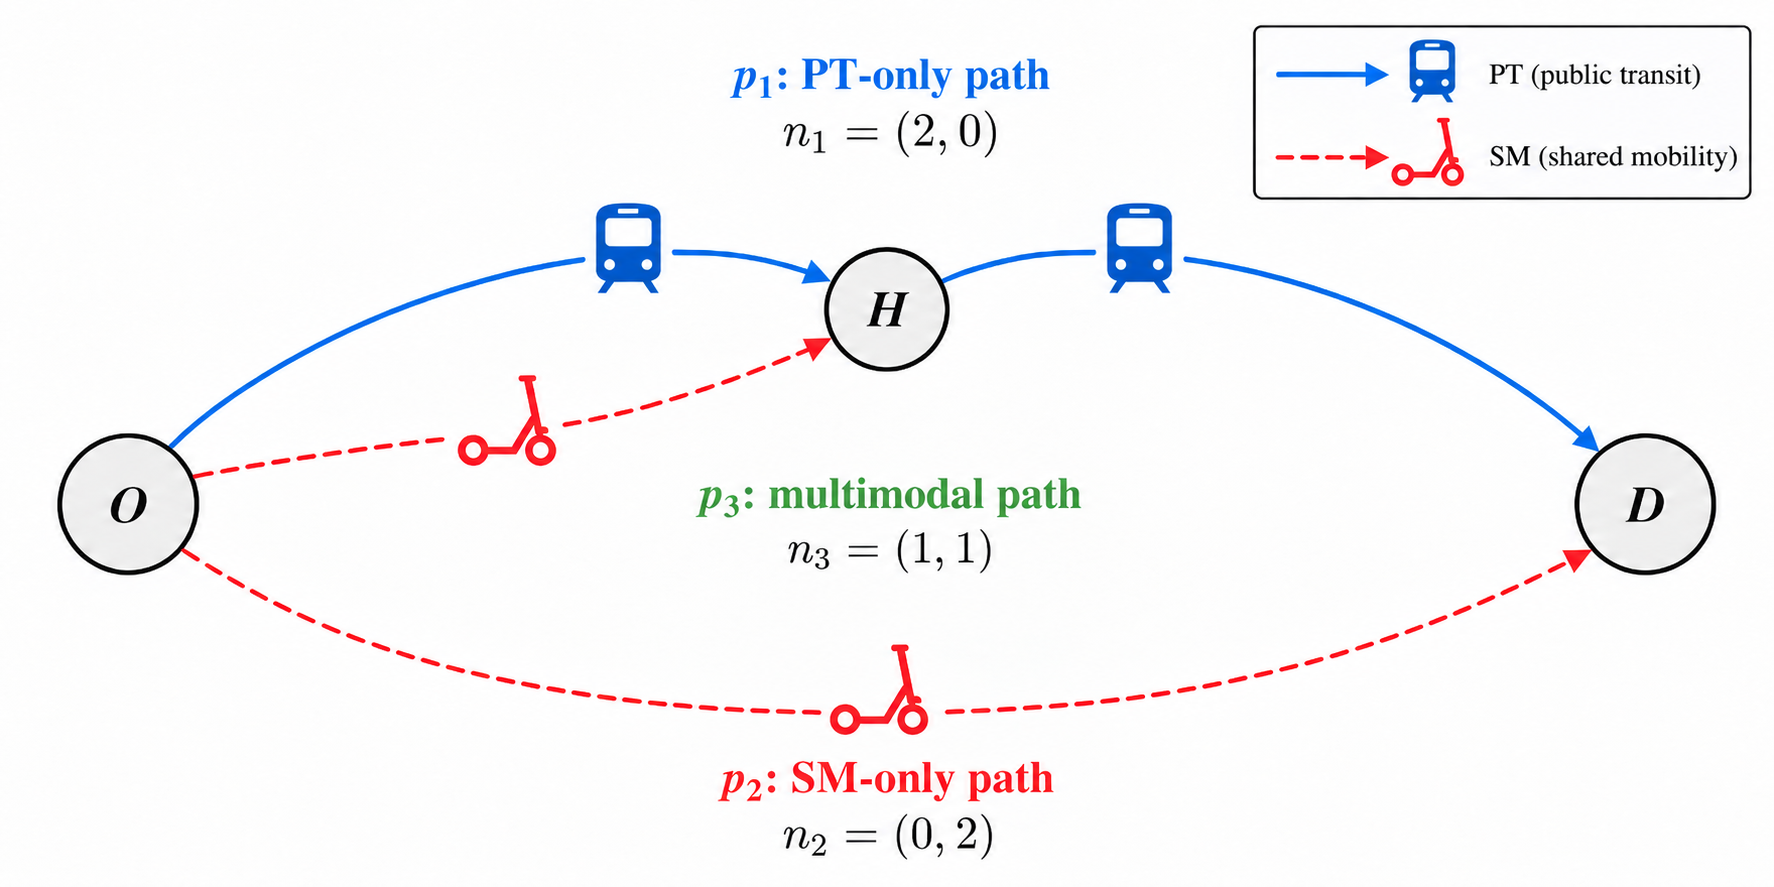
\includegraphics[width=0.68\textwidth]{figures/stylized_network.png}
    \caption{Stylized multimodal network with PT-only, SM-only, and multimodal paths. The unlabeled intermediate node subdivides the SM-only path into two segments, each representing one unit of SM usage.}
    \label{fig:stylized-network}
\end{figure}

The baseline instance contains three traveler classes with path-cost vectors
\begin{equation}
    c_P=(4,5,4.5),\qquad
    c_M=(5,4.5,3),\qquad
    c_S=(5.5,3,4.5),
\end{equation}
and identical trip-frequency distributions
\begin{equation}
    \mu_P,\mu_M,\mu_S\sim U[16,24].
\end{equation}
Their initial population shares are
\begin{equation}
    Q_P=Q_M=Q_S=\frac13.
\end{equation}

The menu contains PAYG and two subscription bundles. The mode-specific overage tariffs and unit provision costs are
\begin{equation}
    \rho=(2,4),
    \qquad
    k=(0.5,1).
\end{equation}
Only parameters directly relevant to the numerical analysis are reported here; complete implementation details and auxiliary settings will be provided with the open-source code.

\subsection{Algorithmic Illustration}

Figure~\ref{fig:stylized-valuation} examines the lower-level valuation structure for traveler class $M$. Panel~(a) shows the EMTC
\begin{equation}
    G_M(\varepsilon)
    =
    \mathbb{E}_{\mu\sim U[16,24]}
    \left[\Phi_M(\mu;\varepsilon)\right].
\end{equation}
The EMTC decreases as either modal allowance increases and approaches the minimum travel-cost level when both allowances become sufficiently large. The non-axis-aligned contours also indicate that the two allowance dimensions are jointly determined through endogenous path substitution.

For a realized trip frequency,
\begin{equation}
    \Phi_M(\mu;\varepsilon)
    =
    \max_{j\in J_M}
    \left\{
        \mu\pi_M^j-(\omega_M^j)^\top\varepsilon
    \right\}.
\end{equation}
Each dual extreme point defines an affine piece of the realized value function, and the allowance space is partitioned according to the active extreme point. Panel~(b) shows these regime boundaries for $\mu=16$, $20$, and $24$.

The partitions exhibit a clear scaling pattern as the realized trip frequency changes. This follows from the positive homogeneity of the lower-level allocation problem:
\begin{equation}
    \Phi_M(\lambda\mu;\lambda\varepsilon)
    =
    \lambda\Phi_M(\mu;\varepsilon),
    \qquad \lambda\geq0,
\end{equation}
or equivalently,
\begin{equation}
    \Phi_M(\mu;\varepsilon)
    =
    \mu\,
    \Phi_M\left(1;\frac{\varepsilon}{\mu}\right).
\end{equation}
Hence, the active dual regime depends on the normalized allowance vector $\varepsilon/\mu$. Different demand realizations therefore generate scaled versions of a common normalized regime partition. Network complexity may alter the shape and number of these regions, while trip-frequency variation rescales the underlying geometry.

This also explains the relation between the two panels. For a fixed allowance vector, different realizations of $\mu$ imply different normalized allowances and may activate different dual regimes. The EMTC in panel~(a) averages over these moving realized-demand partitions, smoothing the sharp regime transitions associated with any single demand realization.

\begin{figure}[t]
    \centering
    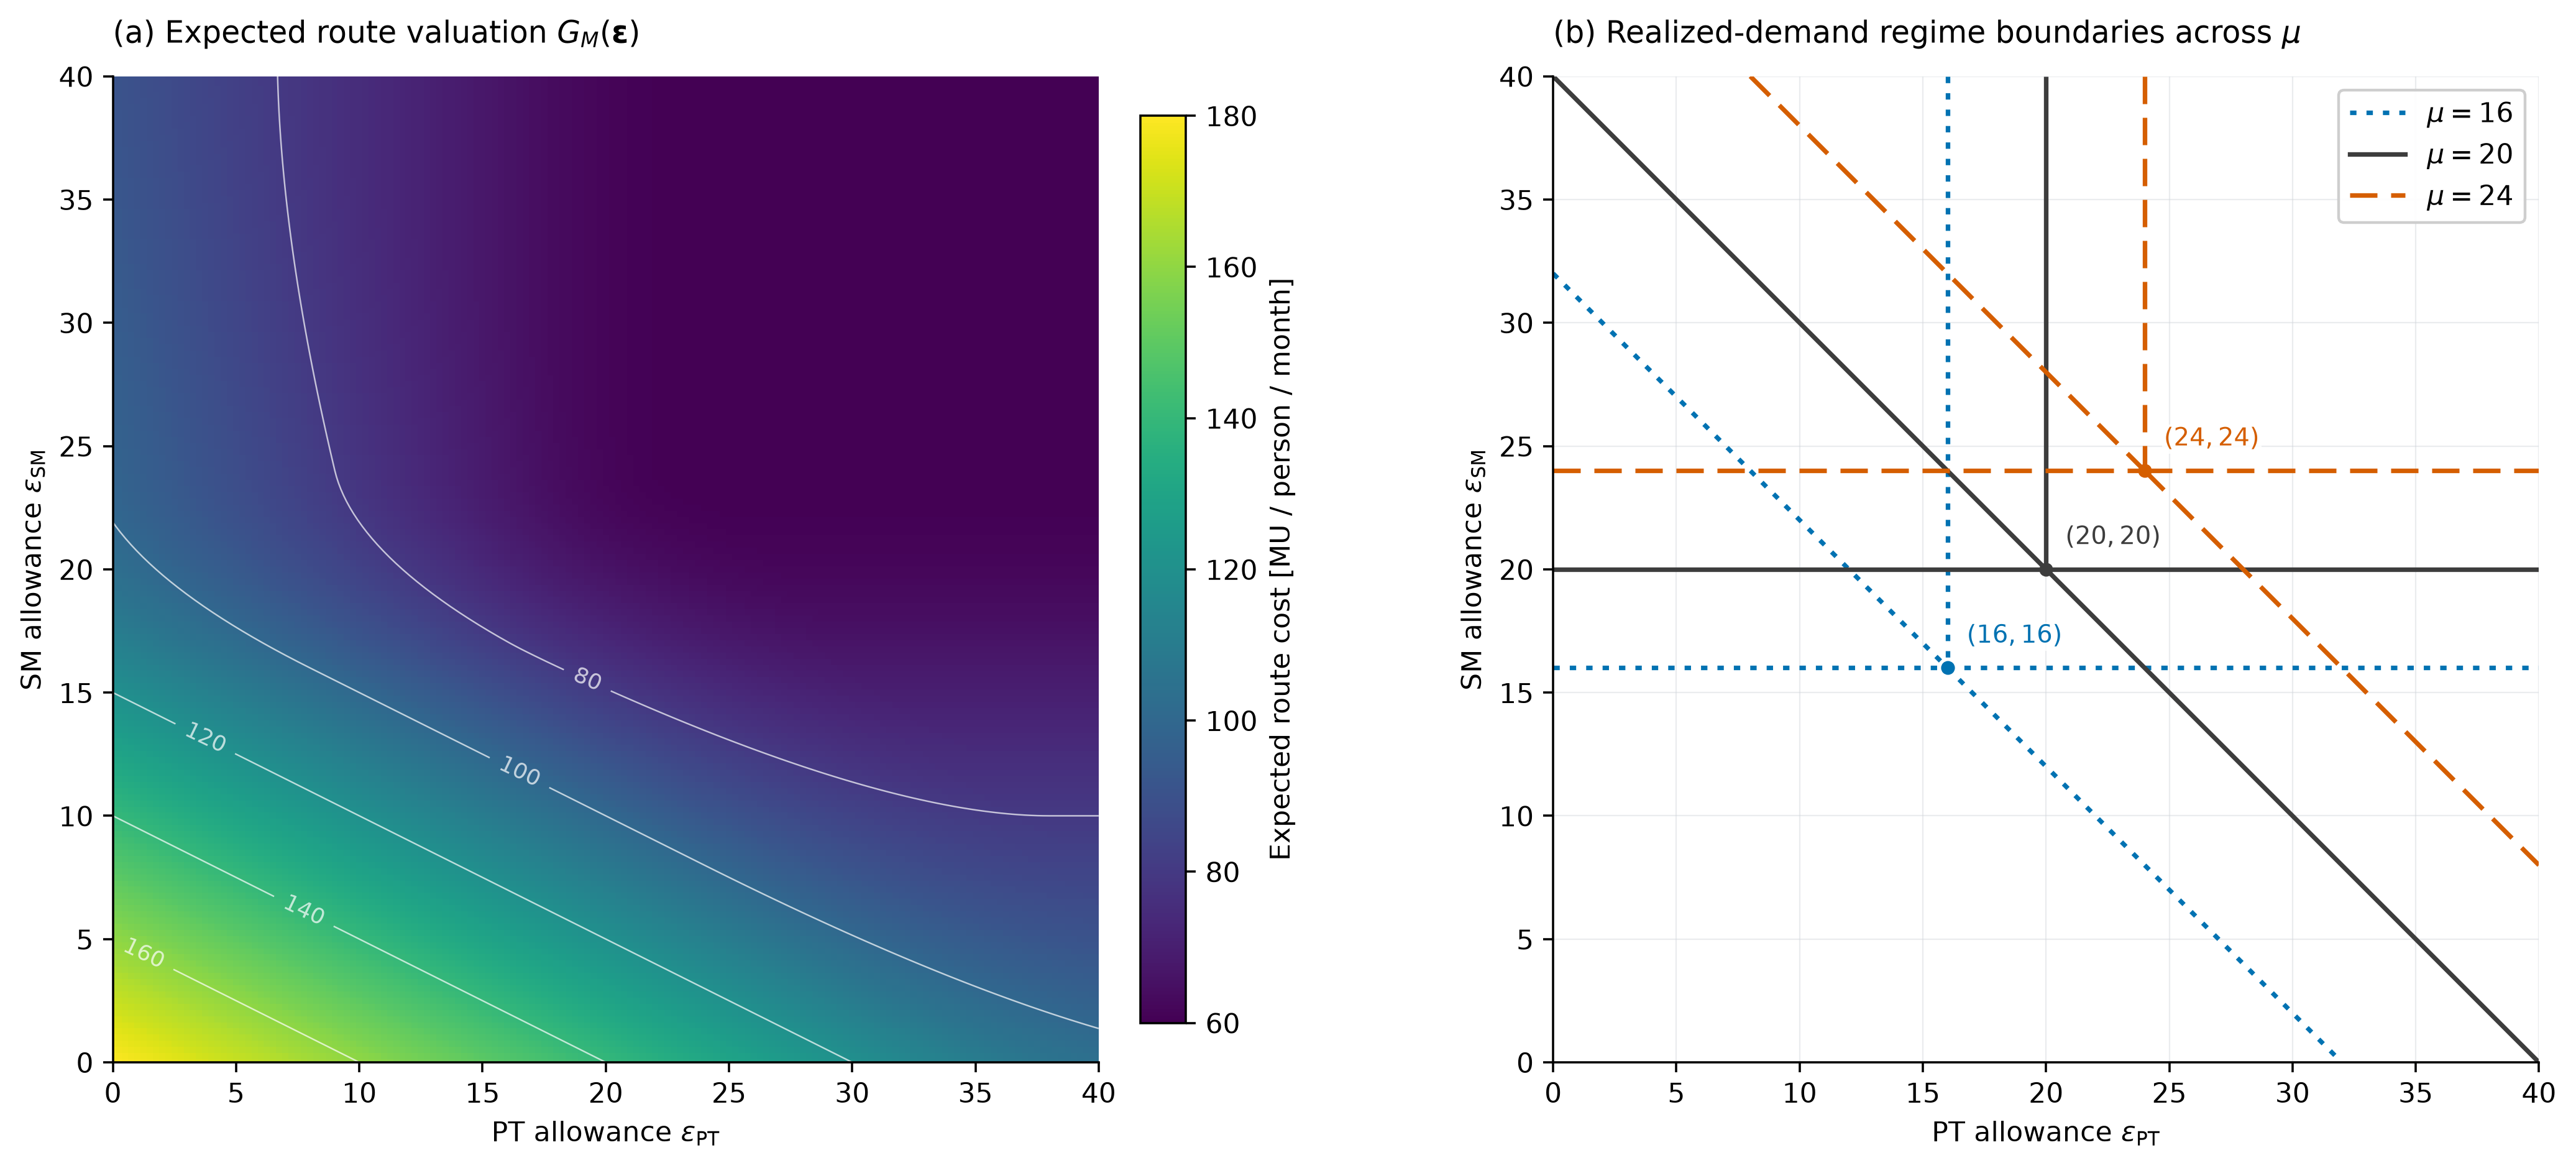
\includegraphics[width=\textwidth]{figures/a1_valuation_structure.png}
    \caption{
    Valuation structure for traveler class $M$.
    Panel~(a) shows the EMTC
    $G_M(\boldsymbol{\varepsilon})$ under
    $\mu\sim U[16,24]$.
    Panel~(b) shows the realized-demand dual-regime boundaries for
    $\mu=16$, $20$, and $24$.
    }
    \label{fig:stylized-valuation}
\end{figure}

\subsection{Bundle-Design Insights}

\subsection{Large-Scale Computational Experiments}

\section{Conclusion}

\small
\Urlmuskip=0mu plus 1mu\relax
\bibliographystyle{abbrvnat}
\bibliography{ref}
\end{document}
